\documentclass{report}

\usepackage{amsmath}
\usepackage{amssymb}
\usepackage{mathrsfs}
\usepackage{graphicx}

\begin{document}
\begin{center}
\textbf{Pong}
\end{center}
\graphicspath{ {./LaTeX1/} }

Étant donné qu’on a défini le vecteur vitesse initial par $\vec{v}(t):(Vx_{init}~t,Vy_{init}~t)$ ou encore $\vec{v}(t)=Vx_{init}~t~\vec{i}~+~Vy_{init}~t~\vec{j}$ alors on peut en déduire la position de la balle en fonction du temps noté $\vec{P}$:\\
$\vec{P}~=~\int\vec{v}(t)dt$\\
$~~~~~$= $(\frac{1}{2}Vx_{init}t^{2}+x_{init})\vec{i}~+~(\frac{1}{2}Vy_{init}t^{2}+y_{init})\vec{j}$\\
\\
Qu’on peut écrire sous forme :\\
$\vec{P}=((\frac{1}{2}Vx_{init}t^{2}+x_{init})\vec{i}~,~(\frac{1}{2}Vy_{init}t^{2}+y_{init})\vec{j})$\\
\\
Cette équation nous permet de décrire la trajectoire de la balle lorsqu’elle ne touche aucun élément du décor. Lorsque la balle touchera un élément $x_{init}$ et $y_{init}$ vont changer par le point d’impact de la balle sur l’élément. Aussi $Vx_{init}$ et $Vy_{init}$ vont changer car la trajectoire ne sera plus la même.\\
On note 3 murs tel que :\\
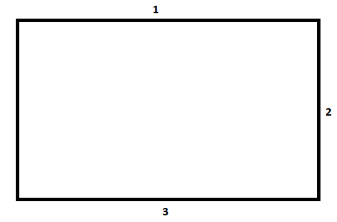
\includegraphics{murs}\\
\\
Ces murs sont des surfaces d’impacts sur lequel la balle doit rebondir. Chaque mur change les coordonnées du vecteur vitesse tel que :\\
Si c’est le mur 1 :\\
$\vec{v}(t):(Vx_{init},\lvert Vy_{init} \rvert)$\\
Si c’est le mur 2 :\\
$\vec{v}(t):(-\lvert Vx_{init} \rvert,Vy_{init})$\\
Si c’est le mur 3 :\\
$\vec{v}(t):(Vx_{init},-\lvert Vy_{init} \rvert)$\\
\\
\\
\\
\\
\\
\\
\\
\\
\\
Lorsque la balle touche la raquette, elle doit ajuster sa trajectoire pour ne pas traverser la raquette. Aussi, cette trajectoire change selon la position de la balle selon la raquette ($coords_{impact}$) . Ainsi le vecteur position de la balle peu être représenté par ce schéma lors du renvoie de la balle par la raquette : \\
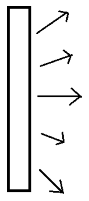
\includegraphics{raquette}\\

$angle = \frac{90}{longueur_{raquette}}*y_{impact}+(45-\frac{90}{longueur_{raquette}}*(x_{raquette}+longueur_{raquette}))$

\end{document}